\documentclass{article}

%Deutsche Sprachunterstützung
\usepackage[utf8]{inputenc}
\usepackage[ngerman]{babel}
\usepackage{marvosym}
\DeclareUnicodeCharacter{20AC}{\EUR}

%Für das Einbinden von Bildern
%\usepackage{graphicx}

%Tabellen
\usepackage{array}

%Tabellen automatisch schoener
\usepackage{booktabs}

%Caption
\usepackage{caption}
\usepackage{subcaption}

%Formeln
\usepackage{mathtools}
\usepackage{amsmath}
\usepackage{amssymb}
\usepackage{amstext}
\usepackage{dsfont}

%\usepackage{mnsymbol}

%Vectorpfeile schöner
\usepackage{esvect}

%Formatierung
\usepackage[T1]{fontenc}
\usepackage{lmodern}
\usepackage{microtype}
%\usepackage[german=guillemets]{csquotes}

%Formatierungsanweisungen
\newcommand{\wichtig}[1]{\underline{\large{#1}}}
\newcommand{\aref}[1]{(s.Abb. \ref{#1})}
\newcommand{\R}{\mathbb{R}}
\newcommand{\K}{\mathbb{K}}
\newcommand{\C}{\mathbb{C}}
\begin{document}
\section{Aufgabe 4}
Das fehlende Bauelement ist eine Spule\\
Messung mit Spule allein:\\
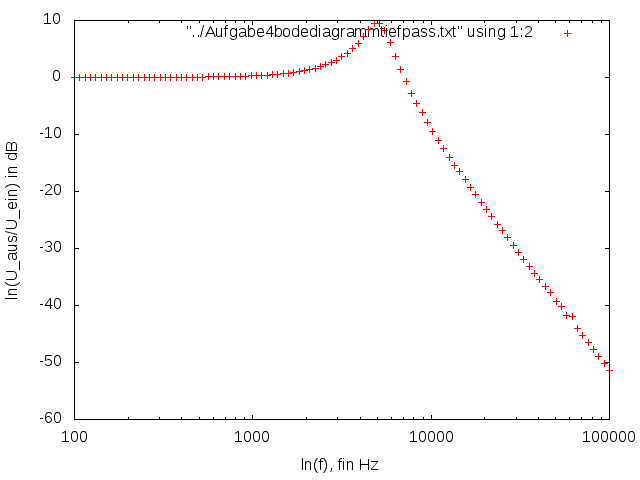
\includegraphics[width=\textwidth]{../daten/Messdaten/plots/Aufgabe4Bodediagramm_tief_gain}
Zweite Messung mit Widerstand in Reihe zur Spule:\\

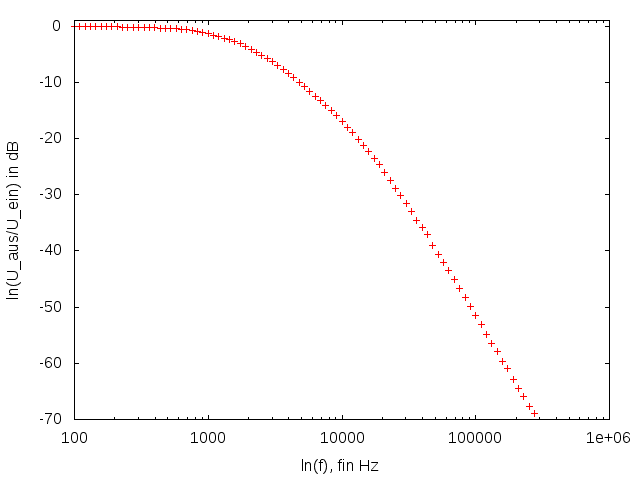
\includegraphics[width=\textwidth]{../daten/Messdaten/plots/Aufgabe4Bodediagramm_tief_R_gain}

\end{document}